\subsection{小模型复测：四阶偏差是否只属于MatterSim？}
旧的小模型测试使用一个MoS$_2$通道和旧QE标签：GRACE兼顾速度与三阶精度，DPA-3.1-3M-FT、Eqnorm三阶误差较小，因此本次优先复测这三者。该选择来自旧样本，并不预设它们的四阶更准确。SevenNet、Nequix及PFT变体在旧单样本三阶测试没有明显优势，本次未扩大到所有旧模型。

本次三模型均采用\textbf{相同PBE DFT弛豫结构和DFPT模式}，三种材料每种五个既定通道，共$3\times3\times181=1629$个构型，保存能量和原子力；最强通道9$\times$9，其余中央5$\times$5。它们是Stage2隔离诊断，不能称为这些小模型自行弛豫的全流程，也不能用来声称全候选排名更好。各通道与既有PBE输入的结构、模态、位移网格和归一化逐项一致；中心13列拟合另以独立最小二乘复核。三模型九条线的重复推理与能量--力差分预检均通过。

\begin{table}[!htbp]\centering\small
\caption{三个小模型对相同PBE构型的误差。三阶为强度误差，四阶为有符号导数误差，单位分别为$\cubunit$、$\quartunit$。符号栏是五个已选通道的符合数，并不是全谱准确率；E为181点中心对齐能量MAE（meV/超胞），F为原子力分量MAE（eV/\AA）。}\label{tab:small-model-metrics}
\allwidthtable{small_model_metrics}\end{table}
\begin{figure}[!htbp]\centering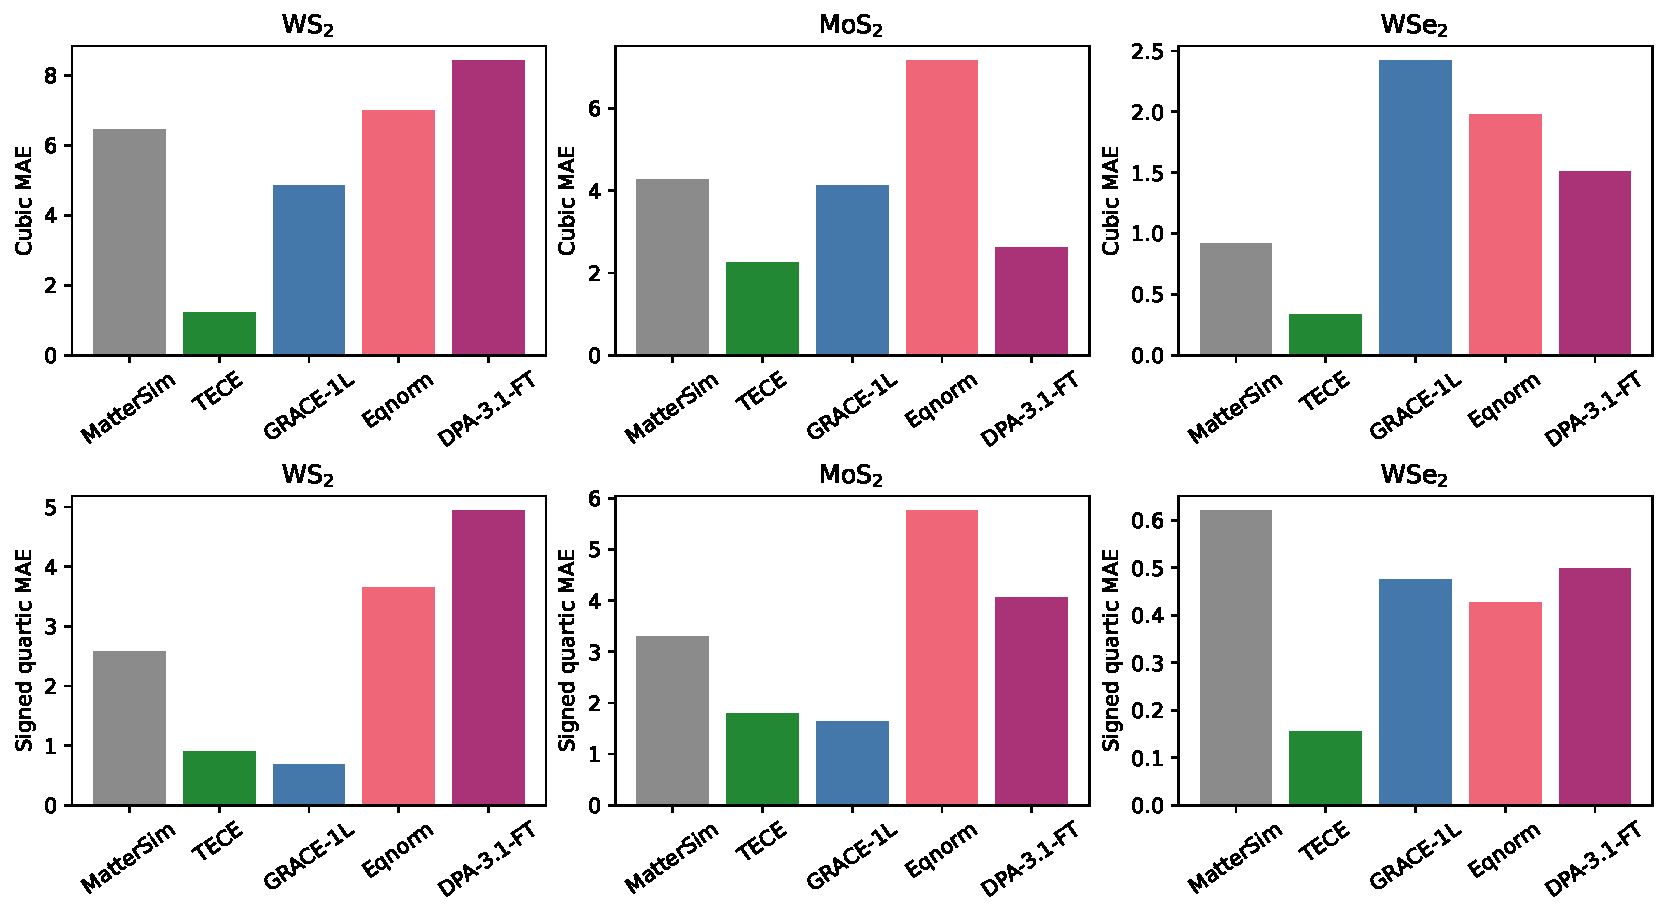
\includegraphics[width=\textwidth]{figures/small_model_errors.pdf}
\caption{固定同一PBE DFT结构和模态时，MatterSim、TECE与三个小模型的三阶强度和有符号四阶MAE。各材料五个通道，排除了Stage1结构与模式的变化。}\label{fig:small-model-errors}\end{figure}

WS$_2$ $\Gamma8$--M6的QE四阶为$-1.4141$，MatterSim为$+1.9304$，TECE为$-1.4250$；GRACE为$-2.9585$、DPA为$+1.6197$、Eqnorm为$+4.4992$。GRACE恢复符号但仍高估负耦合幅度，DPA与Eqnorm同样出现符号错误。因此，\textbf{这个问题不是MatterSim独有，也不是所有MLFF不可避免的缺陷}。不同训练标签、模型势能形状和有限窗口响应都可能影响结果，本实验不能单独确定哪一个训练因素是原因。
\begin{figure}[!htbp]\centering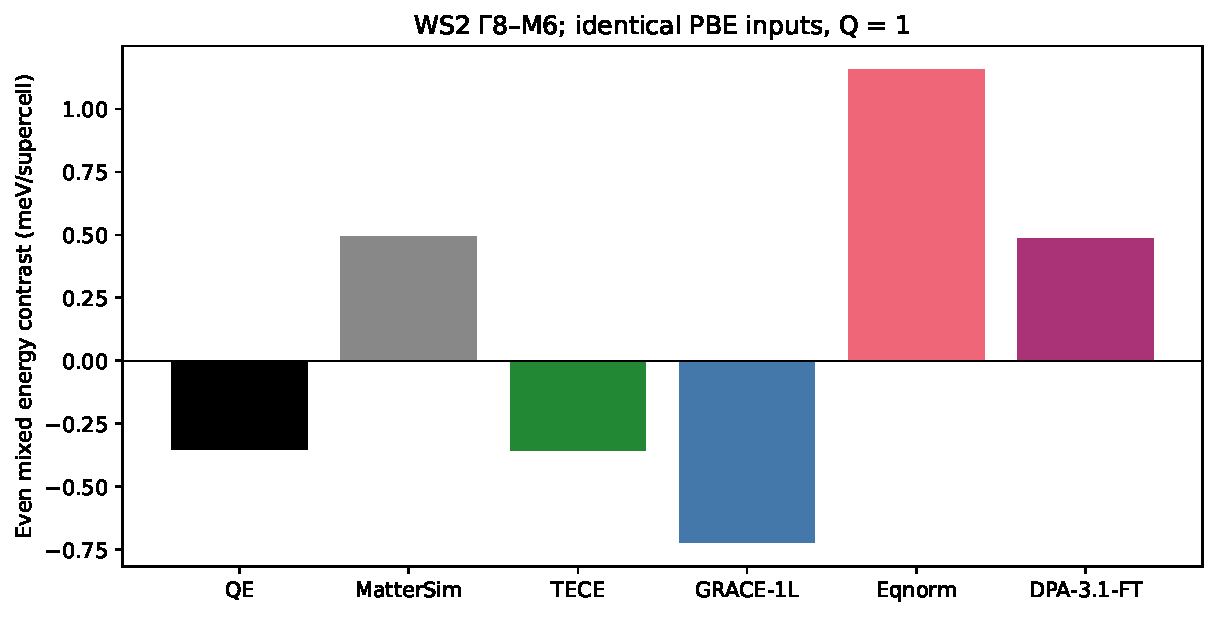
\includegraphics[width=.95\textwidth]{figures/small_model_m6.pdf}
\caption{WS$_2$ $\Gamma8$--M6在$|Q_1|=|Q_2|=1$的偶混合原始能量差。无需多项式拟合就能看到MatterSim、Eqnorm、DPA给出的相互作用方向与QE相反；TECE接近QE，GRACE方向正确但幅度偏大。该量包含更高偶阶项，不等于单独的四阶Taylor系数。}\label{fig:small-model-m6}\end{figure}

GRACE在WS$_2$五通道的四阶MAE为0.675，低于MatterSim的2.572；MoS$_2$为1.642，低于MatterSim的3.302。WSe$_2$三个小模型的四阶MAE均低于MatterSim的0.620，但Eqnorm只在WSe$_2$相对较好，在WS$_2$/MoS$_2$偏差较大。DPA在MoS$_2$三阶MAE为2.607，优于MatterSim的4.274，却没有改善该材料四阶MAE（4.063）。因此三阶准确、整体能量或力误差小，都不能代替对目标四阶项的单独检验。

GRACE在同一服务器CPU配置（8推理线程、独占节点）每种材料181点含加载总耗时约47.7秒，与此前MatterSim约46秒相近；本次不能确认它有显著速度优势。DPA与Eqnorm使用已有本机Apple Silicon环境、2线程，耗时记录仅作来源信息，\textbf{不与服务器作直接速度排名}。旧单样本的GRACE速度优势也不能直接外推到本次完整加载流程。

\begin{table}[!htbp]\centering\scriptsize
\caption{WS$_2$小模型逐通道系数。中央5$\times$5；三阶用强度、四阶保留符号。拟合RMSE为多项式对模型能量的残差（meV/超胞），不等于对QE误差。其余材料逐通道值保存于可复算JSON。}\label{tab:small-model-details}
\allwidthtable{small_model_ws2}\end{table}
本次优先建议将GRACE作为MatterSim的Stage2候选对照，将TECE作为高阶精度对照；没有证据支持把DPA或Eqnorm直接替换为默认Stage2。模型选择需按材料和目标通道验证。除既有WS$_2$最强通道的QE/MatterSim高密度实验外，本次三个小模型未做17$\times$17复算，有限窗口结果不应表述为全部四阶导数已严格收敛。
\FloatBarrier
